\subsection{Caso em que todos os par�metros s�o desconhecidos}

\begin{align*}
P(s) &= \frac{1}{s^2-1}\begin{bmatrix}
s+3 & 2s\\
-2s-4 & s+3
\end{bmatrix}\\
M(s) &= \begin{bmatrix}
\frac{2}{s+2} & 0\\
0 & \frac{1}{s+1}
\end{bmatrix}\\
r_1 &= \textrm{sin}(0.635t) + \textrm{sin}(4.567t)\\
r_2 &= \textrm{sin}(0.1t) + \textrm{sin}(1.1t)
\end{align*}

\subsubsection{Simula��o \#1}

Inicialmente, verificamos o comportamento do sistema para varia��es no
\textbf{par�metro de adapta��o} $\Gamma$.

\bigskip

\begin{align*}
  \gamma &= \HI{20} \,, \textrm{e} \, \HI{5}
\end{align*}

\begin{figure}[H]
  \centering
  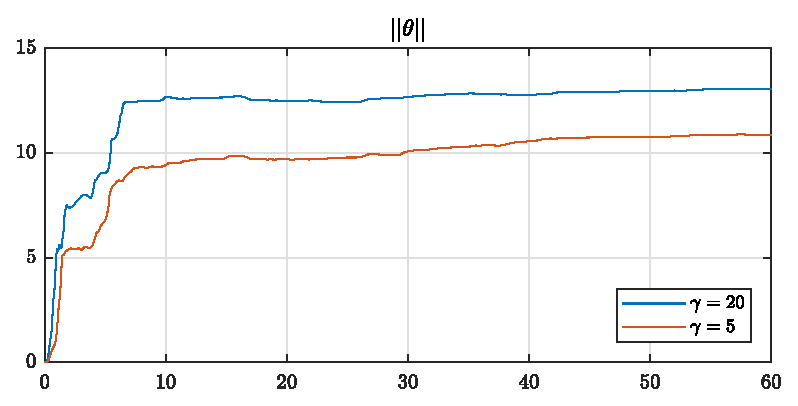
\includegraphics[width=12cm]{figs/2/modtheta/sim0gamma20gamma5.eps}
\end{figure}

\begin{figure}[H]
  \centering
  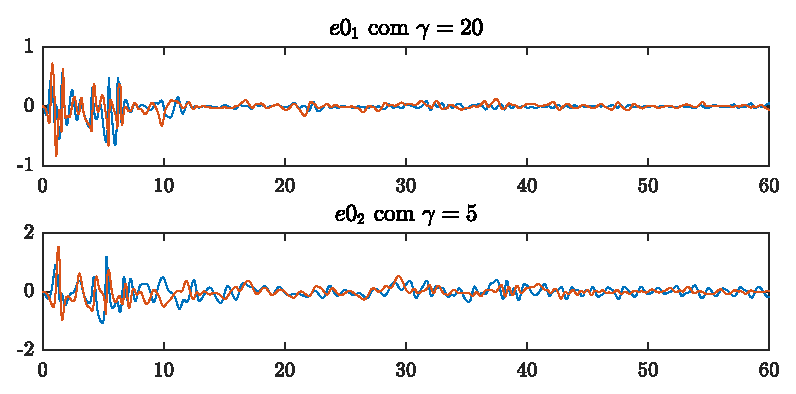
\includegraphics[width=12cm]{figs/2/e0/sim0gamma20gamma5.eps}
\end{figure}

%---------------------------------------------------------------------

\subsubsection{Simula��o \#2}

Verificamos agora o comportamento do sistema para varia��es na \textbf{condi��o inicial} $y(0)$.

\bigskip

\begin{align*}
y0 &= \HI{0} \,, \, \HI{1}
\end{align*}

\begin{figure}[H]
  \centering
  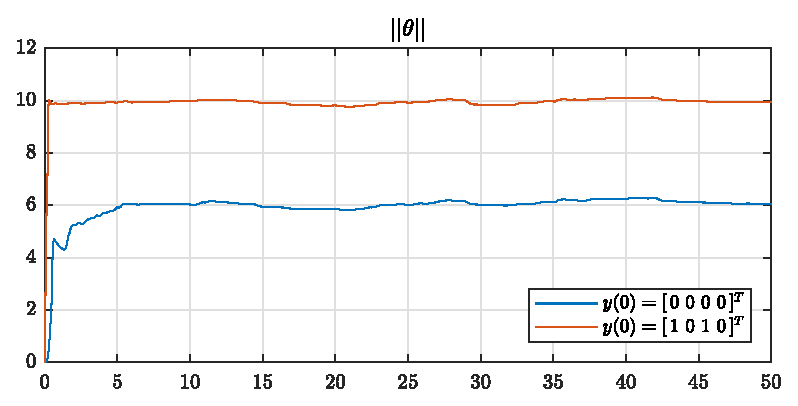
\includegraphics[width=12cm]{figs/2/modtheta/sim0y01y02.eps}
\end{figure}

\begin{figure}[H]
  \centering
  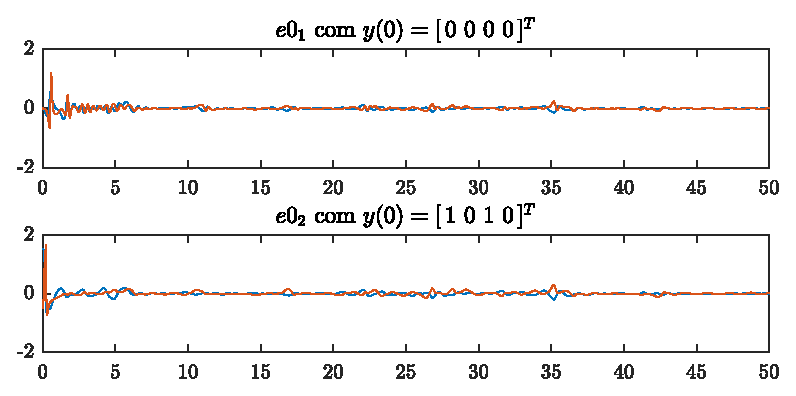
\includegraphics[width=12cm]{figs/2/e0/sim0y01y02.eps}
\end{figure}

% -----------------------------------------------------------------------------

\subsubsection{Simula��o \#3}

Verificamos o comportamento do sistema para varia��es na \textbf{fun��o de transfer�ncia da planta} $P(s)$.

\bigskip

\begin{align*}
	P(s) &= \HI{$\frac{1}{s^2-1}\begin{bmatrix}
	s+3 & s^2 \\
	-2s-4 & s+3
	\end{bmatrix}$} \, \text{e} \, \HI{$\frac{1}{s^2-2s+1}\begin{bmatrix}
	s+2 & s \\
	-s-2 & s+2
	\end{bmatrix}$}
\end{align*}

\begin{align*}
K_p &= \begin{bmatrix}
1 & 1 \\
-1 & 1
\end{bmatrix} \\
d_1 &= 1 > 0 \,, \, d_2 = 2 > 0
\end{align*}

\begin{figure}[H]
  \centering
  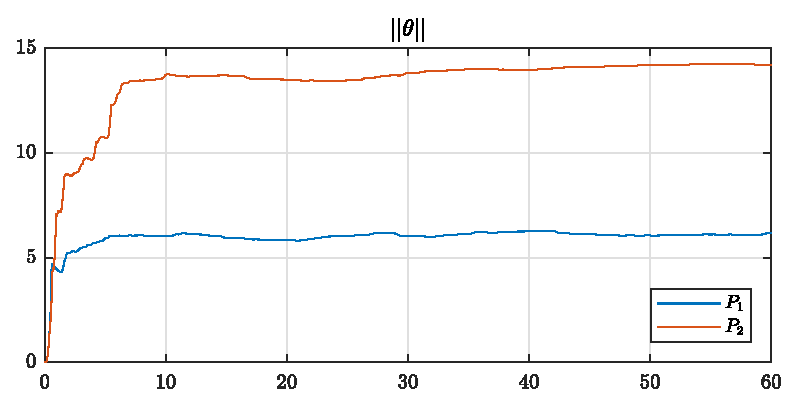
\includegraphics[width=12cm]{figs/2/modtheta/sim0P1P2.eps}
\end{figure}

\begin{figure}[H]
  \centering
  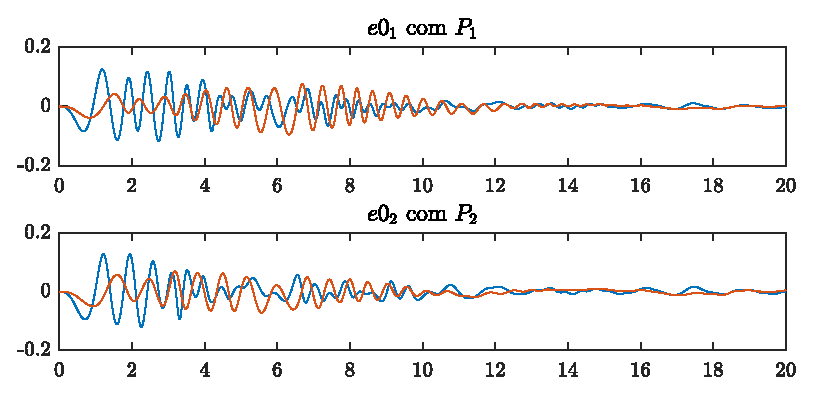
\includegraphics[width=12cm]{figs/2/e0/sim0P1P2.eps}
\end{figure}

% -----------------------------------------------------------------------------

\subsubsection{Simula��o \#4}

Verificamos o comportamento do sistema para varia��es na \textbf{fun��o de
transfer�ncia do modelo de refer�ncia} $P_m(s)$.

\bigskip

\begin{align*}
	M(s) &= \HI{$\begin{bmatrix}
	\frac{2}{s+2} & 0 \\
	0 & \frac{1}{s+1}
	\end{bmatrix}$} \, \text{e} \, \HI{$\begin{bmatrix}
	\frac{1}{s+1} & 0 \\
	0 & \frac{1}{s+1}
	\end{bmatrix}$}
\end{align*}

\begin{figure}[H]
  \centering
  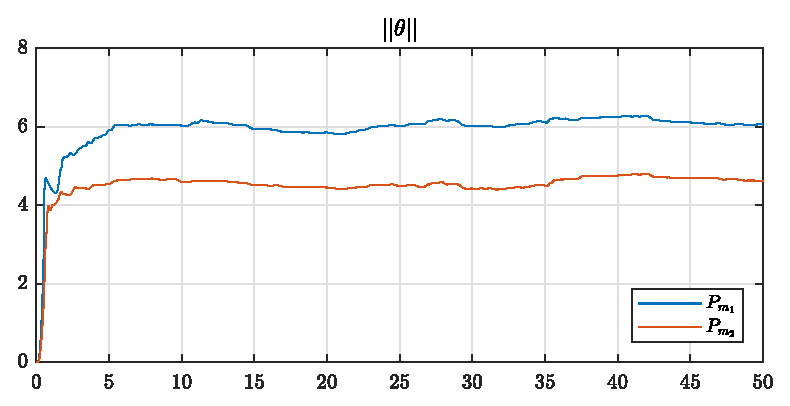
\includegraphics[width=12cm]{figs/2/modtheta/sim0Pm1Pm2.eps}
\end{figure}

\begin{figure}[H]
  \centering
  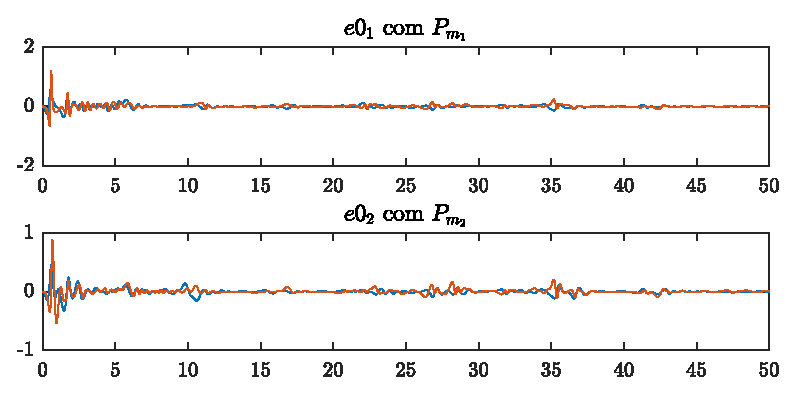
\includegraphics[width=12cm]{figs/2/e0/sim0Pm1Pm2.eps}
\end{figure}
